\section{Техническое задание}
\subsection{Основание для разработки}

Основанием для разработки является задание на выпускную квалификационную работу бакалавра "<Веб-приложение для компьютерной поддержки самостоятельной работы  иностранных студентов при изучении языка программирования  JavaScript">.

\subsection{Цель и назначение разработки}

Основной задачей выпускной квалификационной работы является разработка и внедрение веб-приложения для компьютерной поддержки самостоятельной работы  иностранных студентов при изучении языка программирования  JavaScript.

Посредством внедрения веб-приложения планируется устранить существующие недостатки, связанные с неструктурированным доступом к учебным материалам, отсутствием интерактивных инструментов для практики и тестирования, а также сложностями в организации учебного процесса для иностранных студентов, включая языковые барьеры.

Цель разработки включает следующие подцели:

\begin{itemize}
\item создание единой образовательной платформы для доступа к учебным курсам, урокам и тестам;
\item обеспечение удобного и интуитивно понятного интерфейса для самостоятельного изучения JavaScript;
\item интеграция инструментов для проверки знаний, таких как тесты с автоматической оценкой;
\item оптимизация процессов управления учебным контентом для преподавателей и взаимодействия студентов с платформой.
\end{itemize}

\subsection{Функциональные задачи}

Разрабатываемая веб-платформа включает в себя следующие модули:
\begin{enumerate}
\item {Курсы} — модуль для создания и управления учебными курсами, включающими уроки и тесты. Преподаватели могут добавлять, редактировать и удалять курсы, а студенты получают доступ к материалам.
\item {Уроки} — система управления учебным контентом, позволяющая структурировать материалы курса (текст, изображения, видео) и задавать порядок уроков. Поддерживается предпросмотр уроков и их редактирование.
\item {Тесты} — модуль для создания и прохождения интерактивных тестов. Преподаватели могут задавать вопросы и варианты ответов, а студенты проходят тесты с автоматической оценкой результатов.
\item {Результаты тестов} — инструмент для анализа успеваемости студентов. Преподаватели могут просматривать, удалять и управлять результатами тестов, включая статистику по студентам.
\item {Панель управления преподавателя} — интерфейс для управления курсами, уроками, тестами и результатами, с удобной навигацией и виджетами для быстрого доступа.
\item {Профиль пользователя} — модуль для управления учетной записью, включая настройки аватара и персональной информации.
\item {Сообщения} — система уведомлений для обратной связи (например, сообщения об успешном добавлении урока или удалении результатов).
\item {Панель управления} — страница с виджетами всех вышеперечисленных сервисов.
\end{enumerate}

\subsection{Требования пользователя к интерфейсу web-сайта}

Платформа должна обеспечивать:
\begin{itemize}
    \item авторизацию;
    \item интуитивно понятную навигацию между модулями;
    \item адаптивный интерфейс для десктопных и мобильных устройств.
\end{itemize}

Композиция интерфейса пользователя представлена на рисунках ~\ref{templ:image1}, ~\ref{templ:image2}, ~\ref{templ:image3}, ~\ref{templ:image4}, ~\ref{templ:image5}, ~\ref{templ:image6}, ~\ref{templ:image7}, ~\ref{templ:image8}, ~\ref{templ:image9},  ~\ref{templ:image10}.
\newpage  

Композиция шаблона курсы представлена на рисунке ~\ref{templ:image1} и состоит из:

\begin{itemize}
	\item приветственное окно (1);
	\item окно курса (2);
	\item кнопка для просмотра (3);
	\item окно с ролью авторизованного пользователя (4);
	\item кнопка для создания курса (5);
	\item кнопка для просмотра созданных курсов (6);
	\item кнопка для выхода из профиля (7);
	\item кнопка для смены темы оформления (8).
\end{itemize}

\begin{figure}[h]
	\centering
	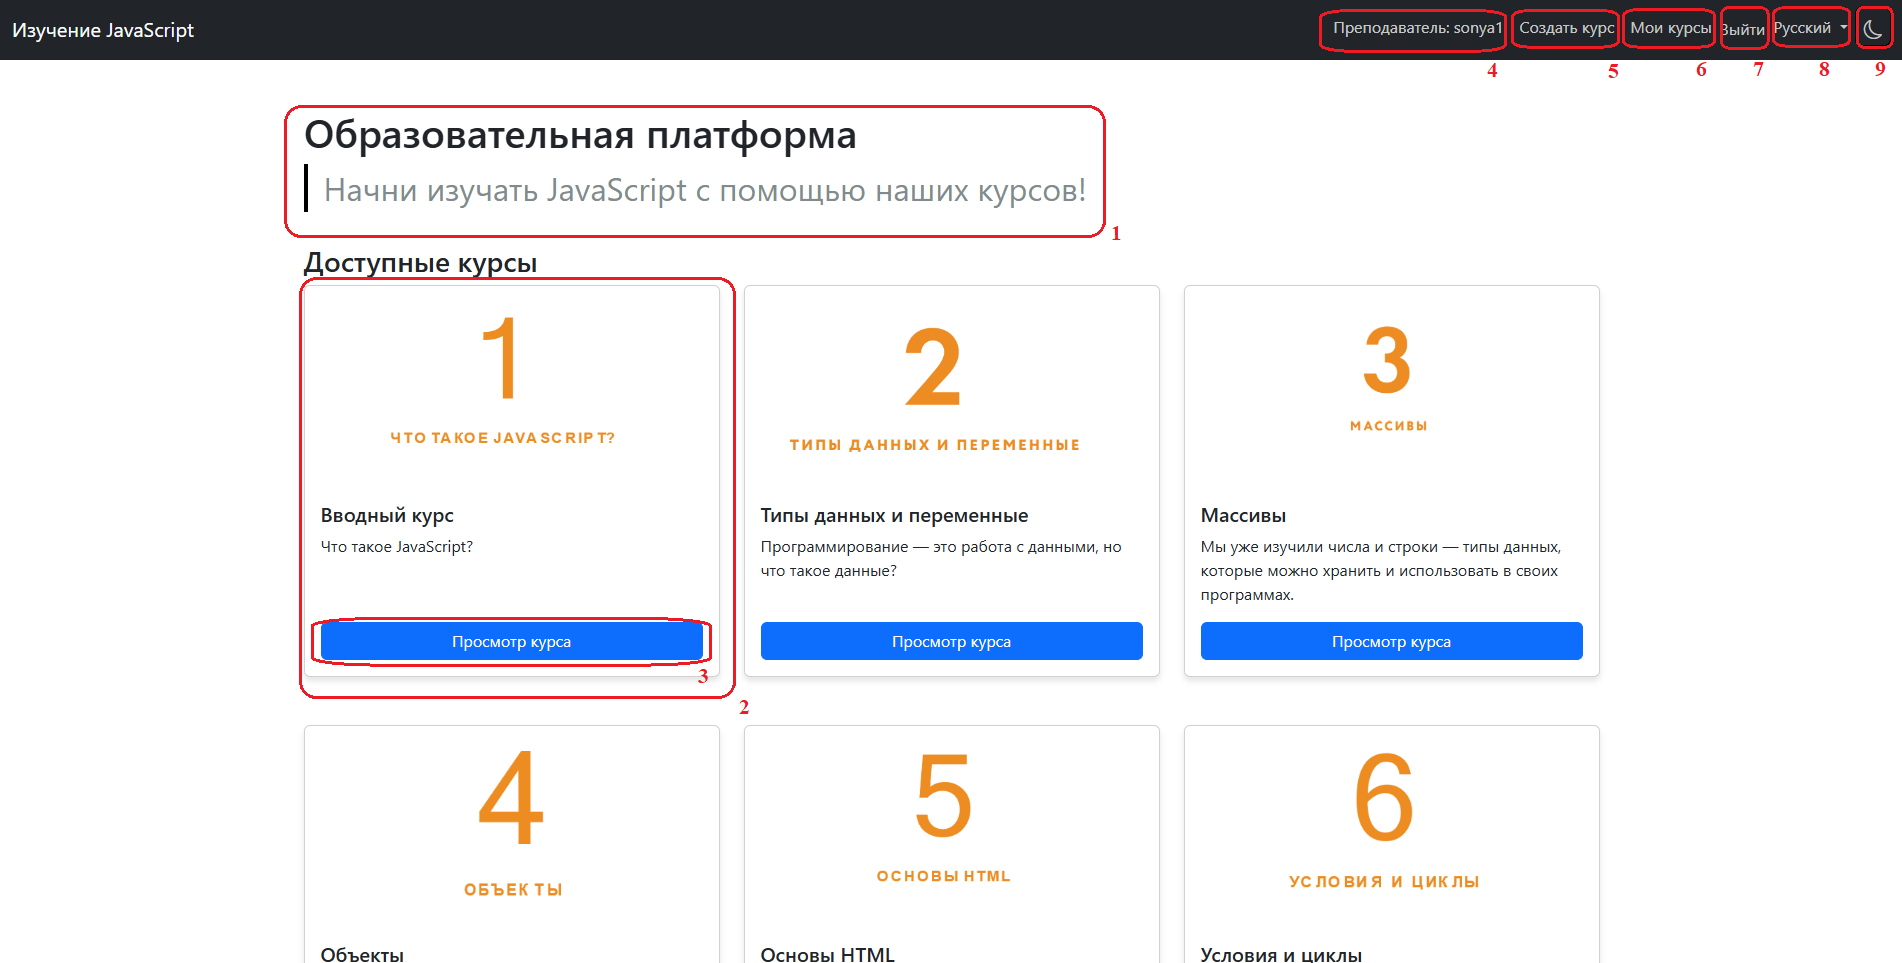
\includegraphics[width=1\linewidth]{images/курсы}
	\caption{Композиция интерфейса сервиса <<Курсы>>}
	\label{templ:image1}
\end{figure}

Композиция шаблона панель управления преподавателя представлена на рисунке ~\ref{templ:image2} и состоит из:

\begin{itemize}
	\item навигационная панель (1);
	\item окно курса (2);
	\item кнопка для редактирования курса (3);
	\item кнопка для просмотра уроков (4);
	\item кнопка для просмотра курса (5);
	\item кнопка для удаления курса (6).
\end{itemize}

\begin{figure}[h]
	\centering
	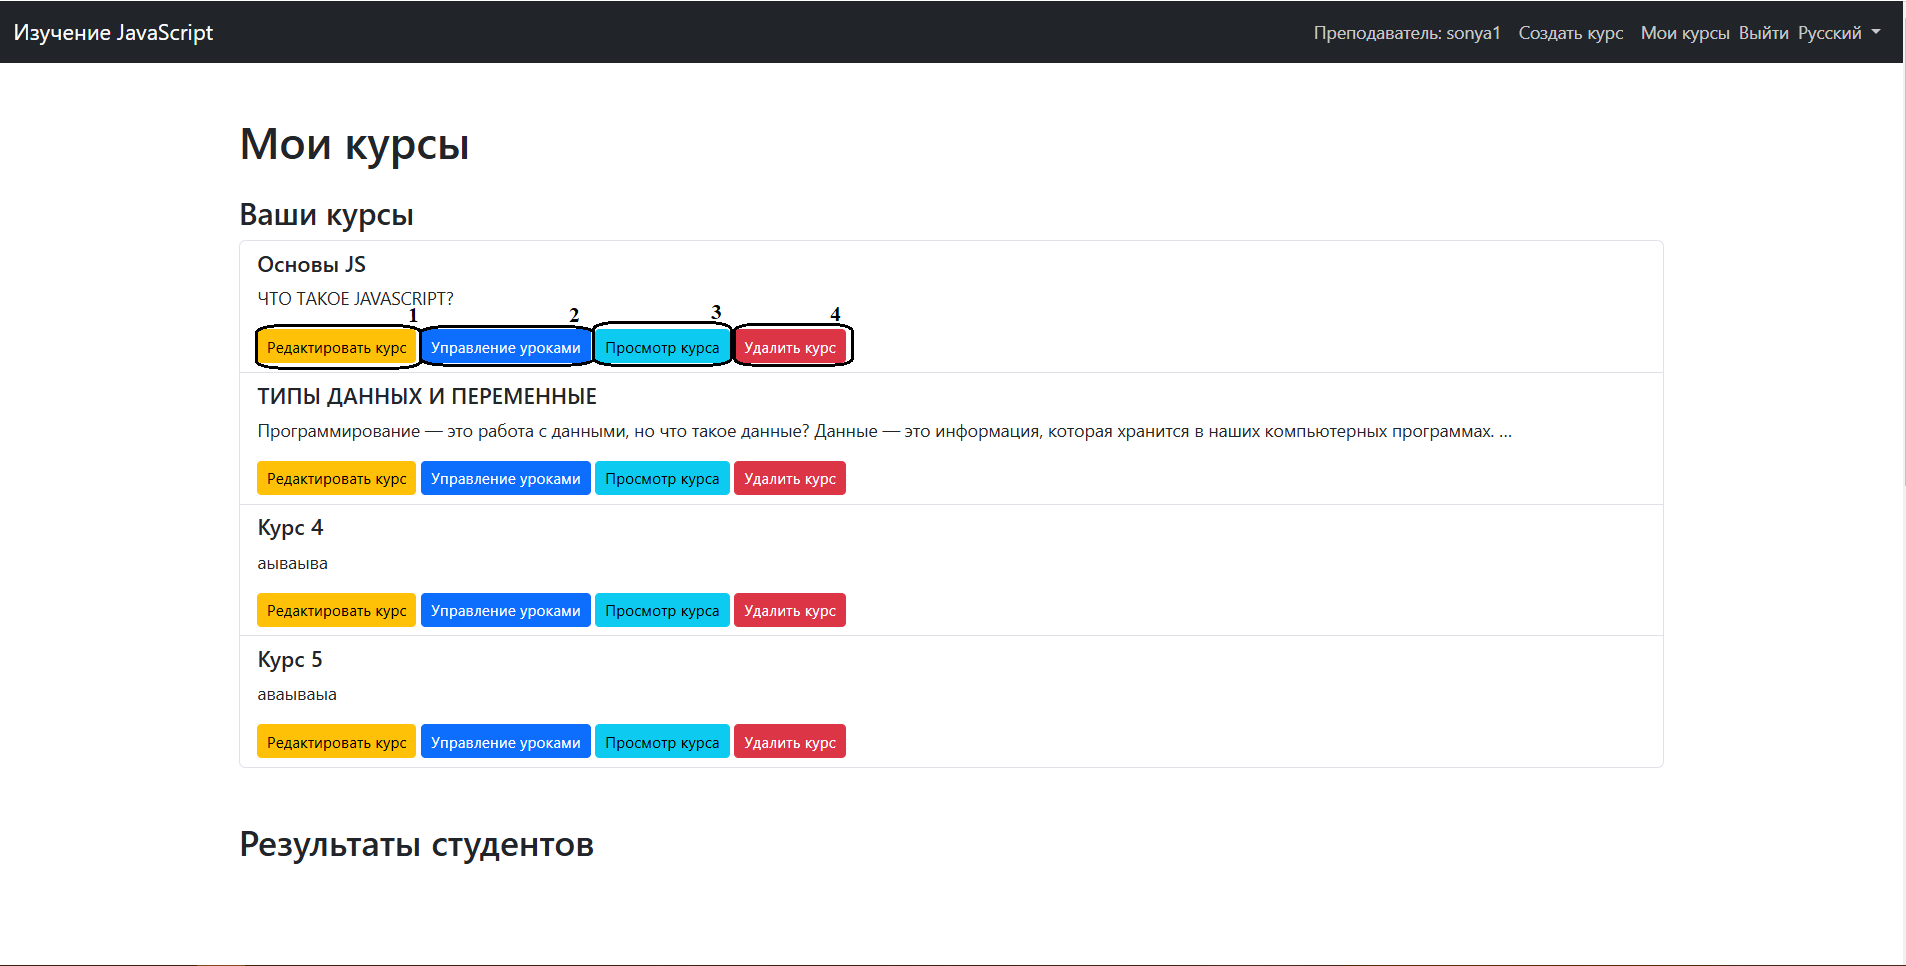
\includegraphics[width=1\linewidth]{images/учитель}
	\caption{Композиция интерфейса сервиса <<Панель управления преподавателя>>}
	\label{templ:image2}
\end{figure}
 

Композиция шаблона уроки представлена на рисунке ~\ref{templ:image3} и состоит из:

\begin{itemize}
	\item навигационная панель (1);
	\item поле с информацией о деталях курса (2);
	\item окно урока (3);
	\item кнопка просмотра урока (4).
\end{itemize}

\begin{figure}[h]
	\centering
	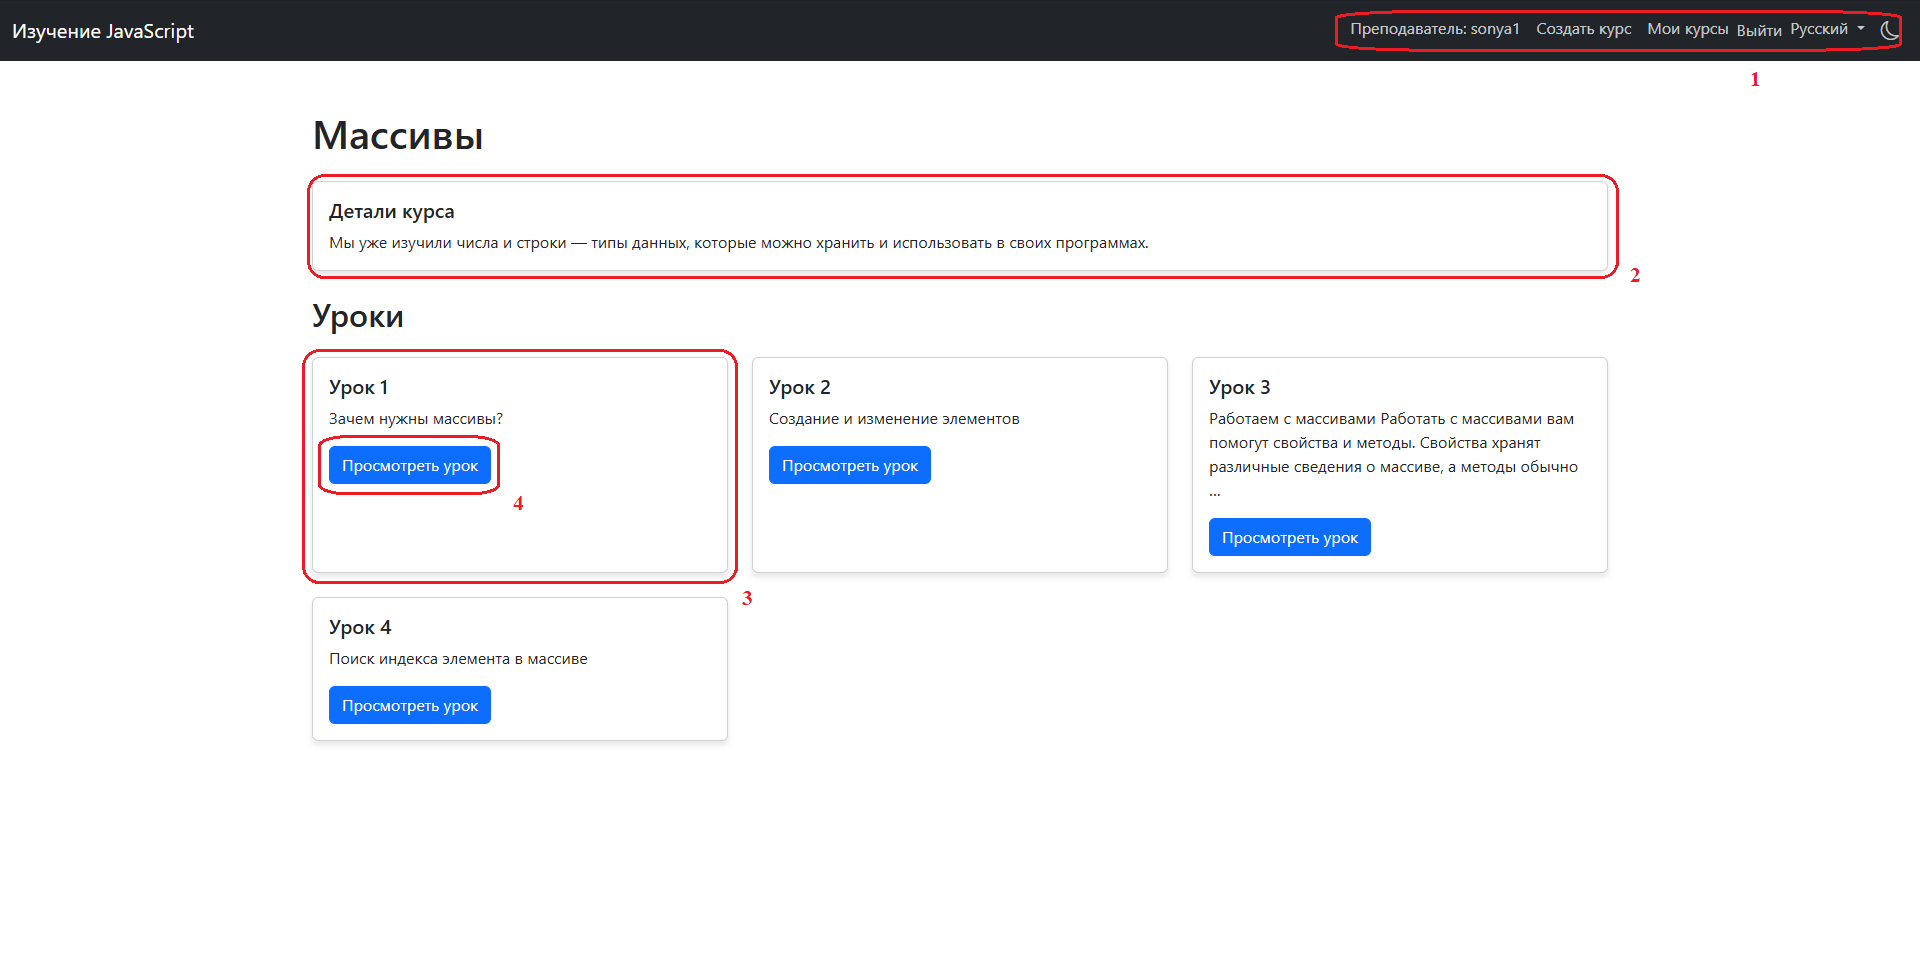
\includegraphics[width=1\linewidth]{images/уроки}
	\caption{Композиция интерфейса сервиса <<Уроки>>}
	\label{templ:image3}
\end{figure}

Композиция шаблона урок представлена на рисунке ~\ref{templ:image4} и состоит из:

\begin{itemize}
	\item навигационная панель (1);
	\item поле с информацией урока (2);
	\item кнопка далее (3);
	\item кнопка назад (4).
\end{itemize}

\begin{figure}[h]
	\centering
	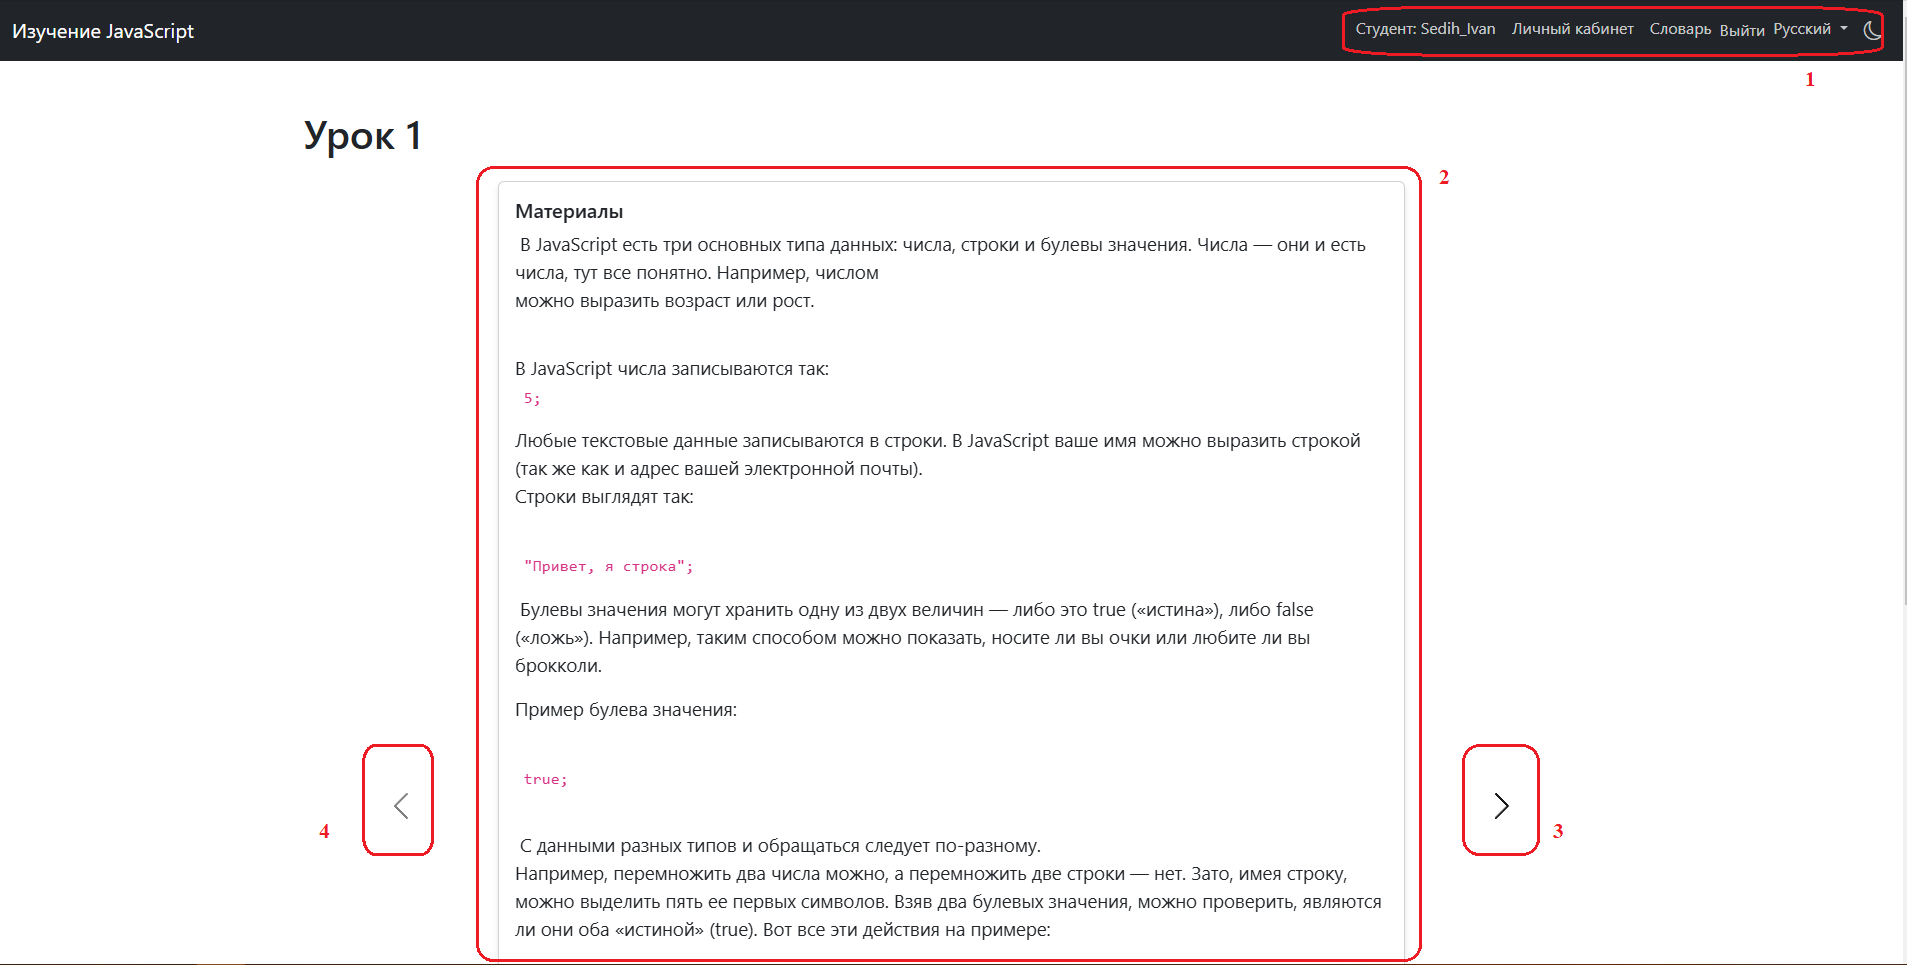
\includegraphics[width=1\linewidth]{images/урок}
	\caption{Композиция интерфейса сервиса <<Урок>>}
	\label{templ:image4}
\end{figure}
\newpage
Композиция шаблона тесты представлена на рисунке ~\ref{templ:image5} и состоит из:

\begin{itemize}
	\item кнопка управления вопросами теста (1);
	\item кнопка управления результатами теста (2);
	\item кнопка удаления теста (3);
	\item поле урока (4);
	\item кнопка добавить тест (5).
\end{itemize}

\begin{figure}[h]
	\centering
	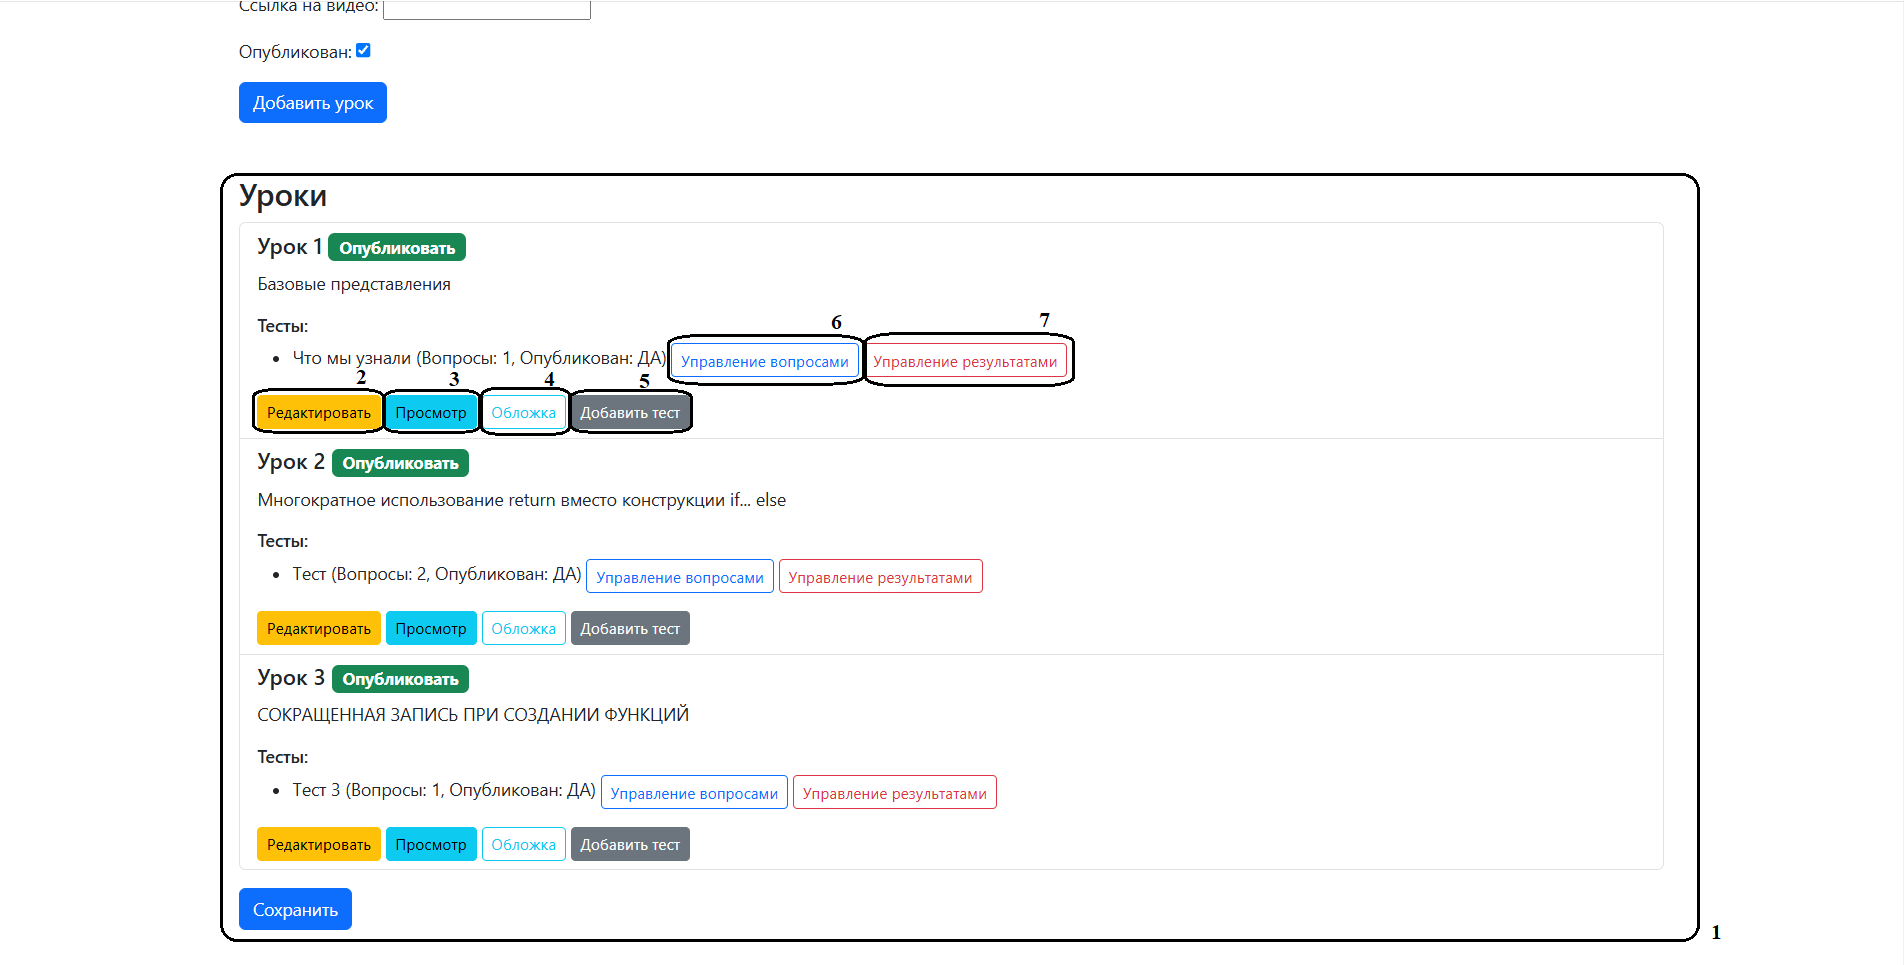
\includegraphics[width=1\linewidth]{images/Тесты}
	\caption{Композиция интерфейса сервиса <<Тесты>>}
	\label{templ:image5}
\end{figure}

Композиция шаблона создание теста представлена на рисунке ~\ref{templ:image6} и состоит из:

\begin{itemize}
	\item навигационная панель (1);
	\item поле создания теста (2);
	\item поле ввода заголовка теста (3);
	\item поле ввода описания теста (4);
	\item поле выбора минимального балла (5);
	\item поле выбора статуса теста (6);
	\item кнопка создания теста (7);
	\item кнопка возврата к урокам (8).
\end{itemize}

\begin{figure}[h]
	\centering
	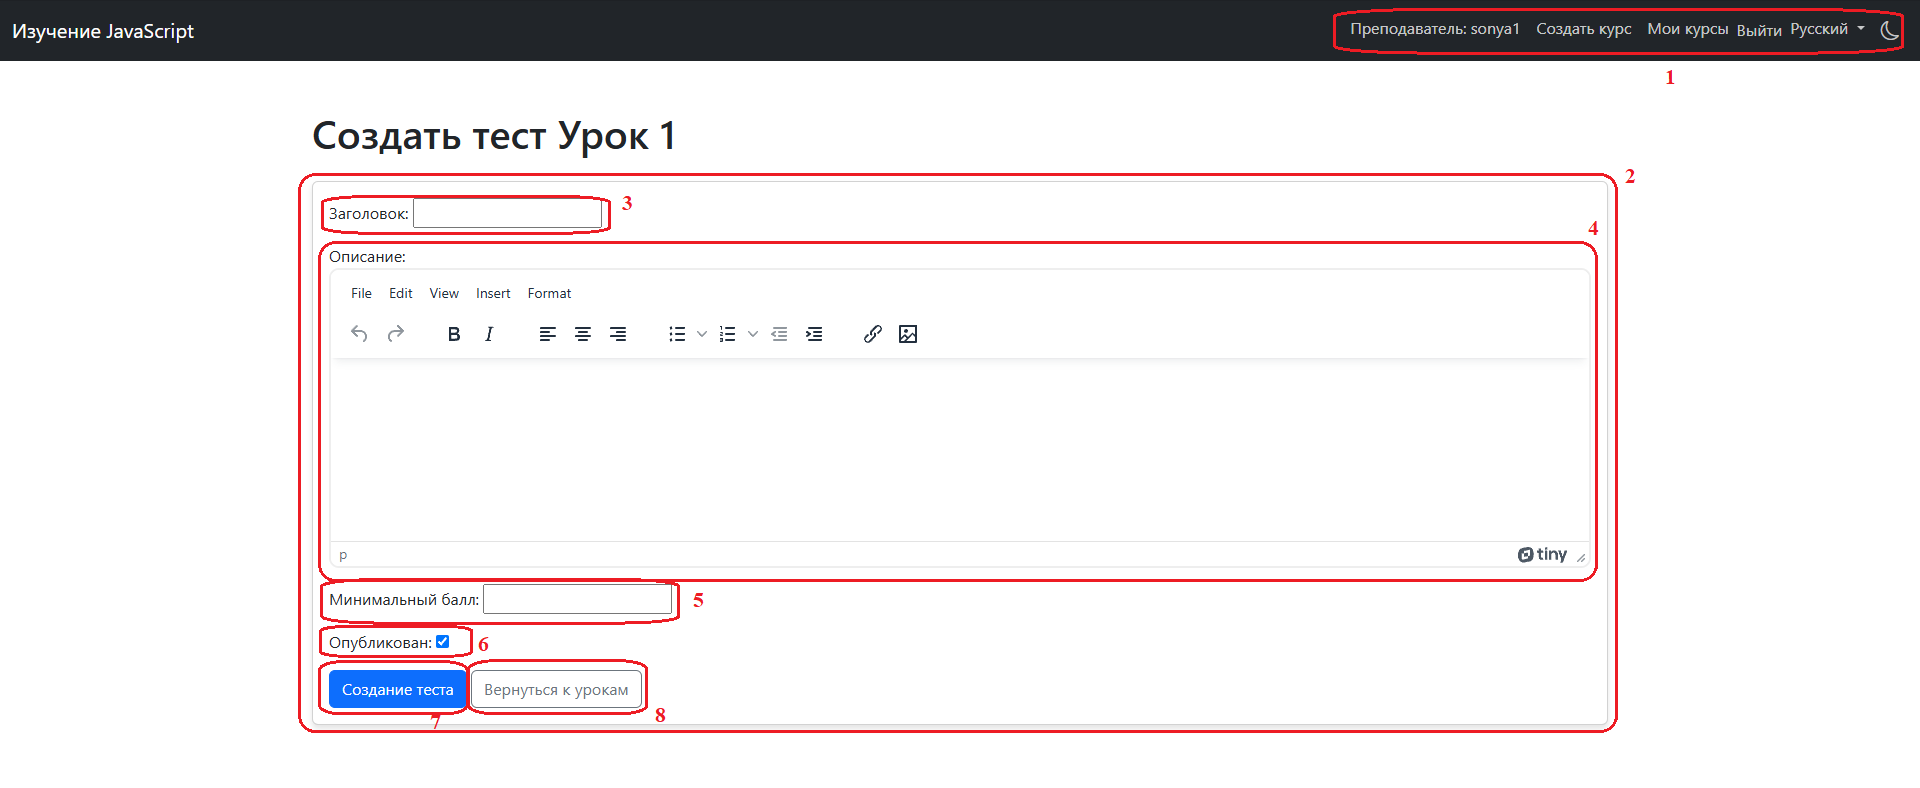
\includegraphics[width=1\linewidth]{images/создатьтест}
	\caption{Композиция интерфейса сервиса <<Создание теста>>}
	\label{templ:image6}
\end{figure}

\newpage
Композиция шаблона результаты теста представлена на рисунке ~\ref{templ:image7} и состоит из:

\begin{itemize}
	\item навигационная панель (1);
	\item поле с информацией о результатах теста (2);
	\item кнопка удалить все результаты (3);
	\item кнопка удалить результат (4);
	\item кнопка вернуться к вопросам (5);
	\item кнопка вернуться к урокам (6).
\end{itemize}

\begin{figure}[h]
	\centering
	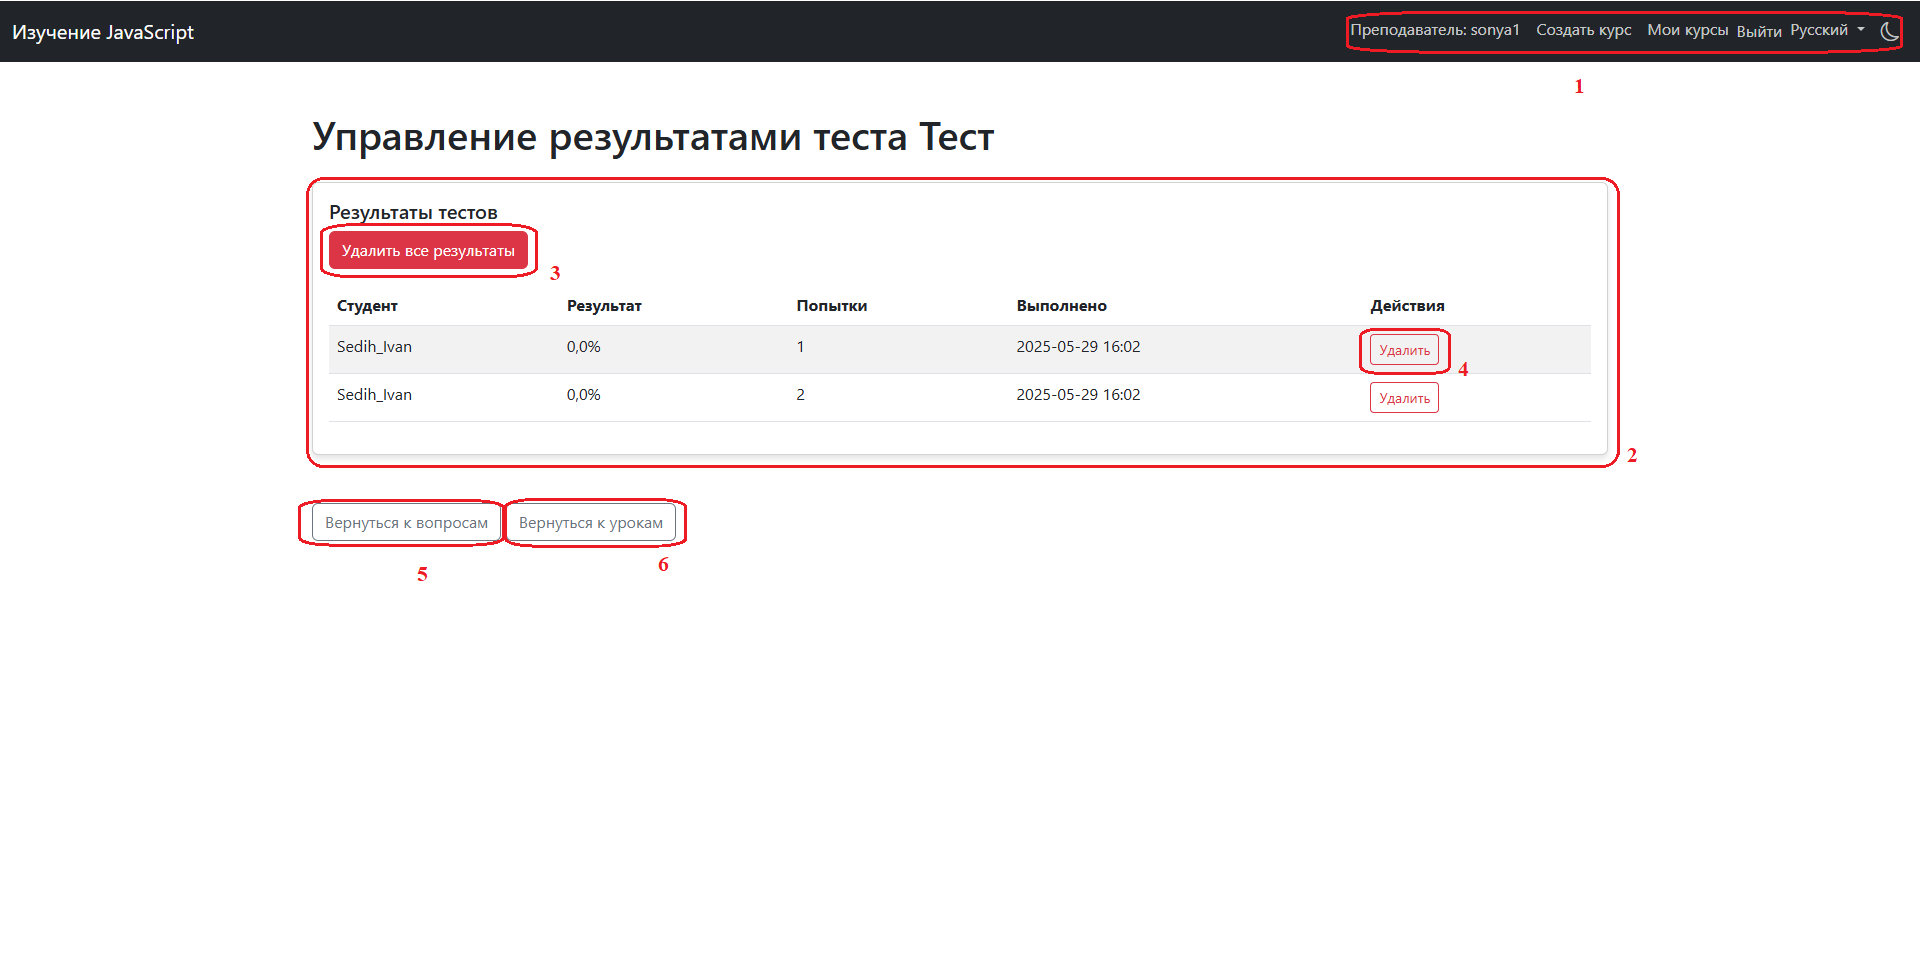
\includegraphics[width=1\linewidth]{images/результаты}
	\caption{Композиция интерфейса сервиса <<Результаты тестов>>}
	\label{templ:image7}
\end{figure}

Композиция шаблона окна авторизации представлена на рисунке ~\ref{templ:image8} и состоит из:

\begin{itemize}
	\item кнопка входа в профиль (1);
	\item кнопка регистрации как студента (2);
	\item кнопка регистрации как преподавателя (3);
	\item кнопка для смены языка (4);
	\item кнопка смены темы оформления (5);
	\item поле входа в профиль (6);
	\item поле ввода имения пользователя (7);
	\item поле ввода пароля (8);
	\item кнопка войти (9).
\end{itemize}

\begin{figure}[h]
	\centering
	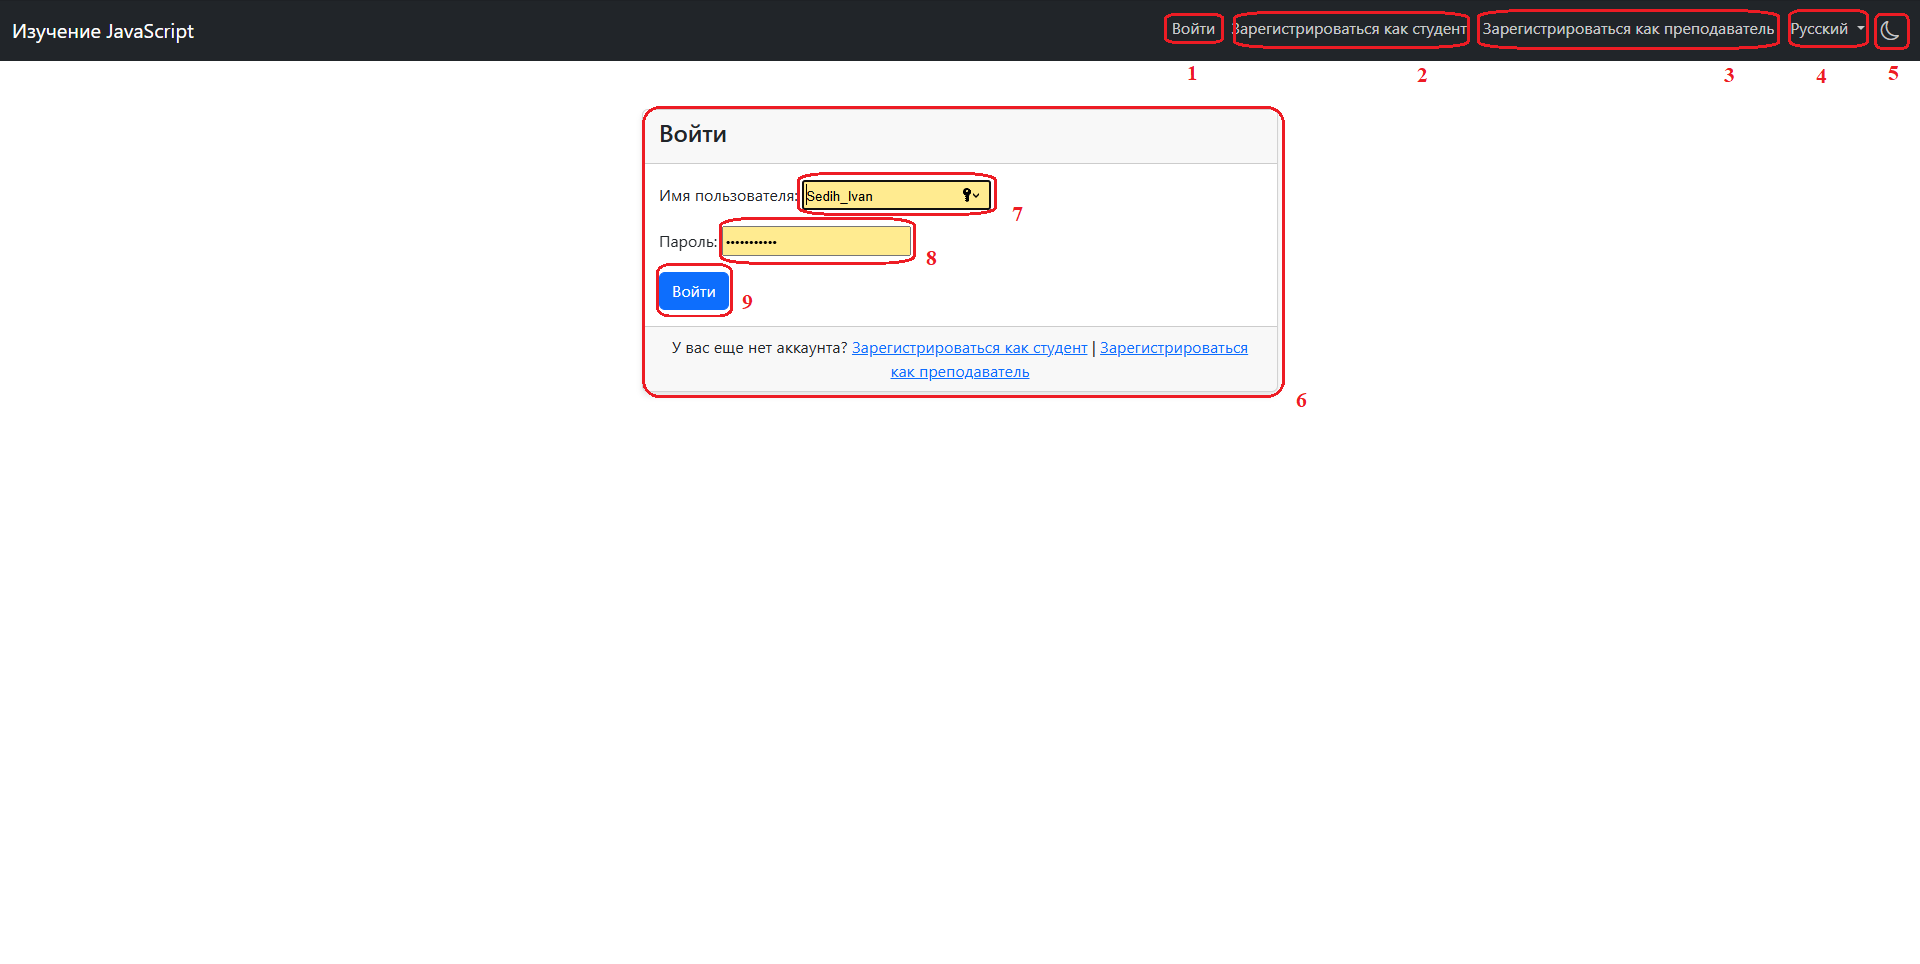
\includegraphics[width=1\linewidth]{images/Авторизация}
	\caption{Композиция интерфейса сервиса <<Авторизация>>}
	\label{templ:image8}
\end{figure}

Композиция шаблона профиль представлена на рисунке ~\ref{templ:image9} и состоит из:

\begin{itemize}
	\item окно с информацией (1);
	\item навигационная панель (2);
	\item поле с аналитической информацией (3);
	\item поле с информацией о курсах (4);
	\item поле с информацией о прогрессе (5);
	\item поле с информацией о достижениях (6).
\end{itemize}

\begin{figure}[h]
	\centering
	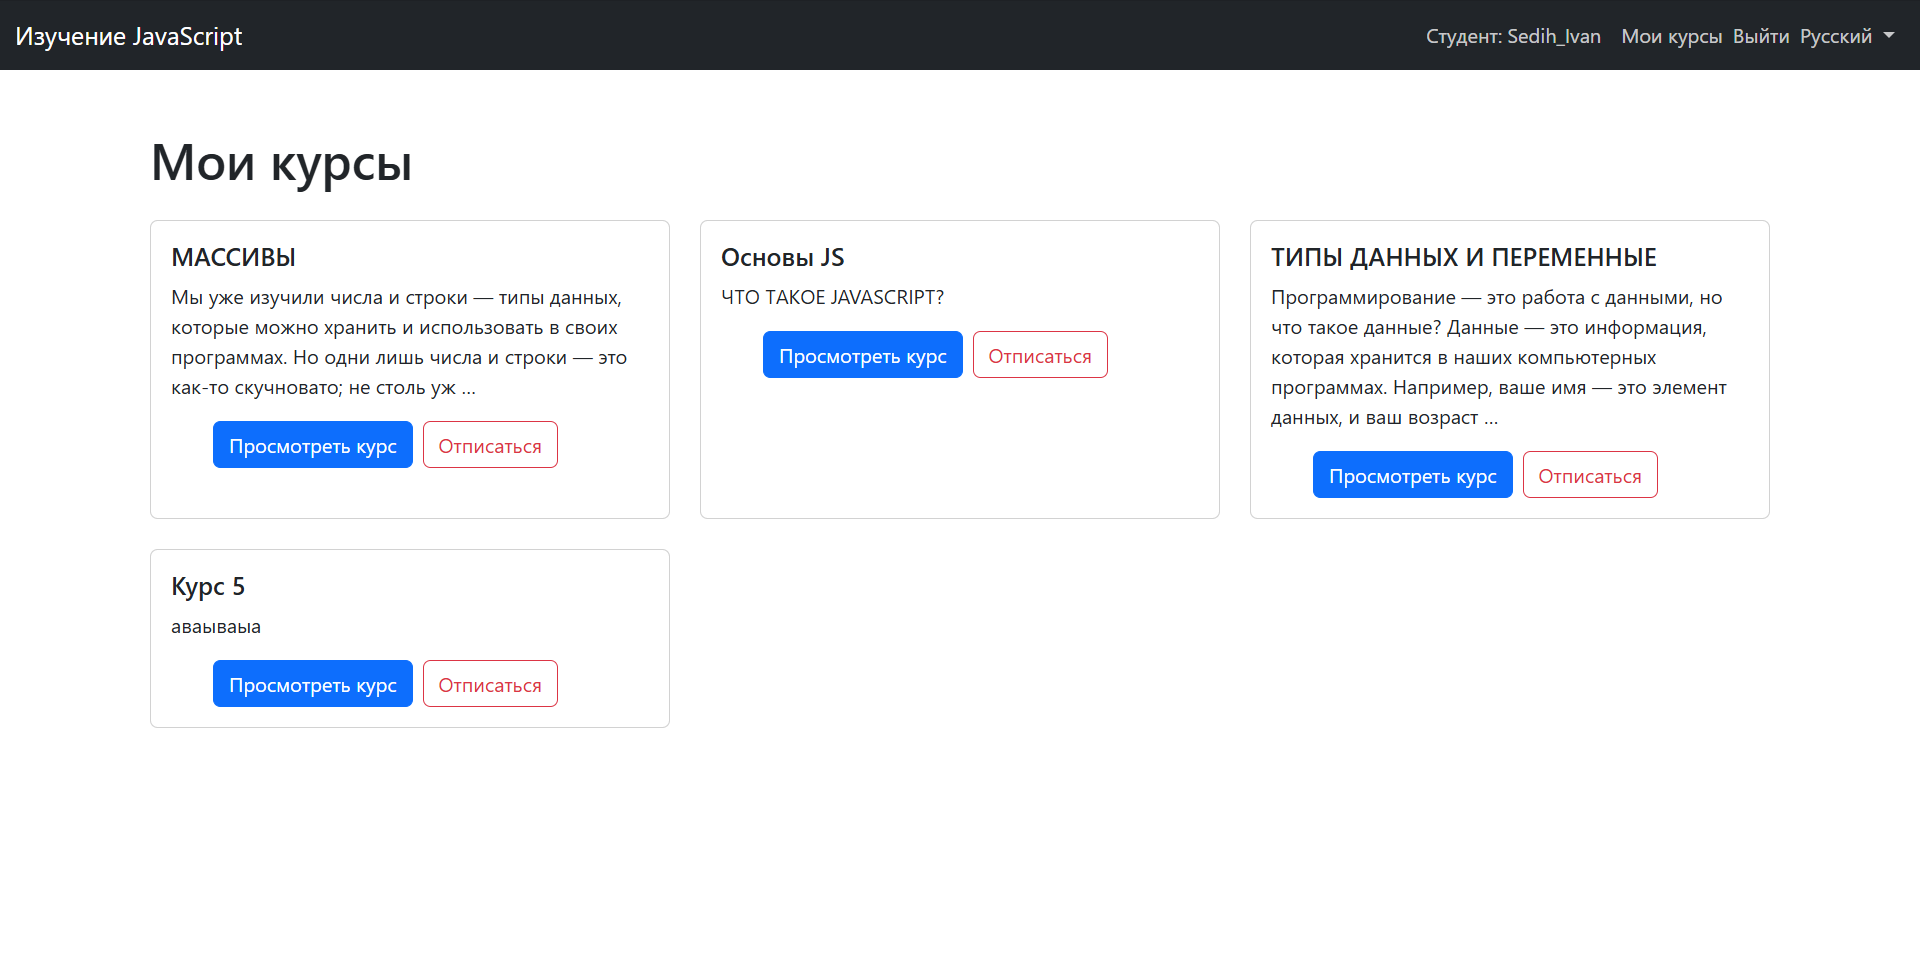
\includegraphics[width=1\linewidth]{images/профиль}
	\caption{Композиция интерфейса сервиса <<Профиль>>}
	\label{templ:image9}
\end{figure}

Композиция шаблона словарь представлена на рисунке ~\ref{templ:image10} и состоит из:

\begin{itemize}
	\item поле ввода термина (1);
	\item окно с информацией о термине (2);
	\item навигационная панель (3).
\end{itemize}

\begin{figure}[h]
	\centering
	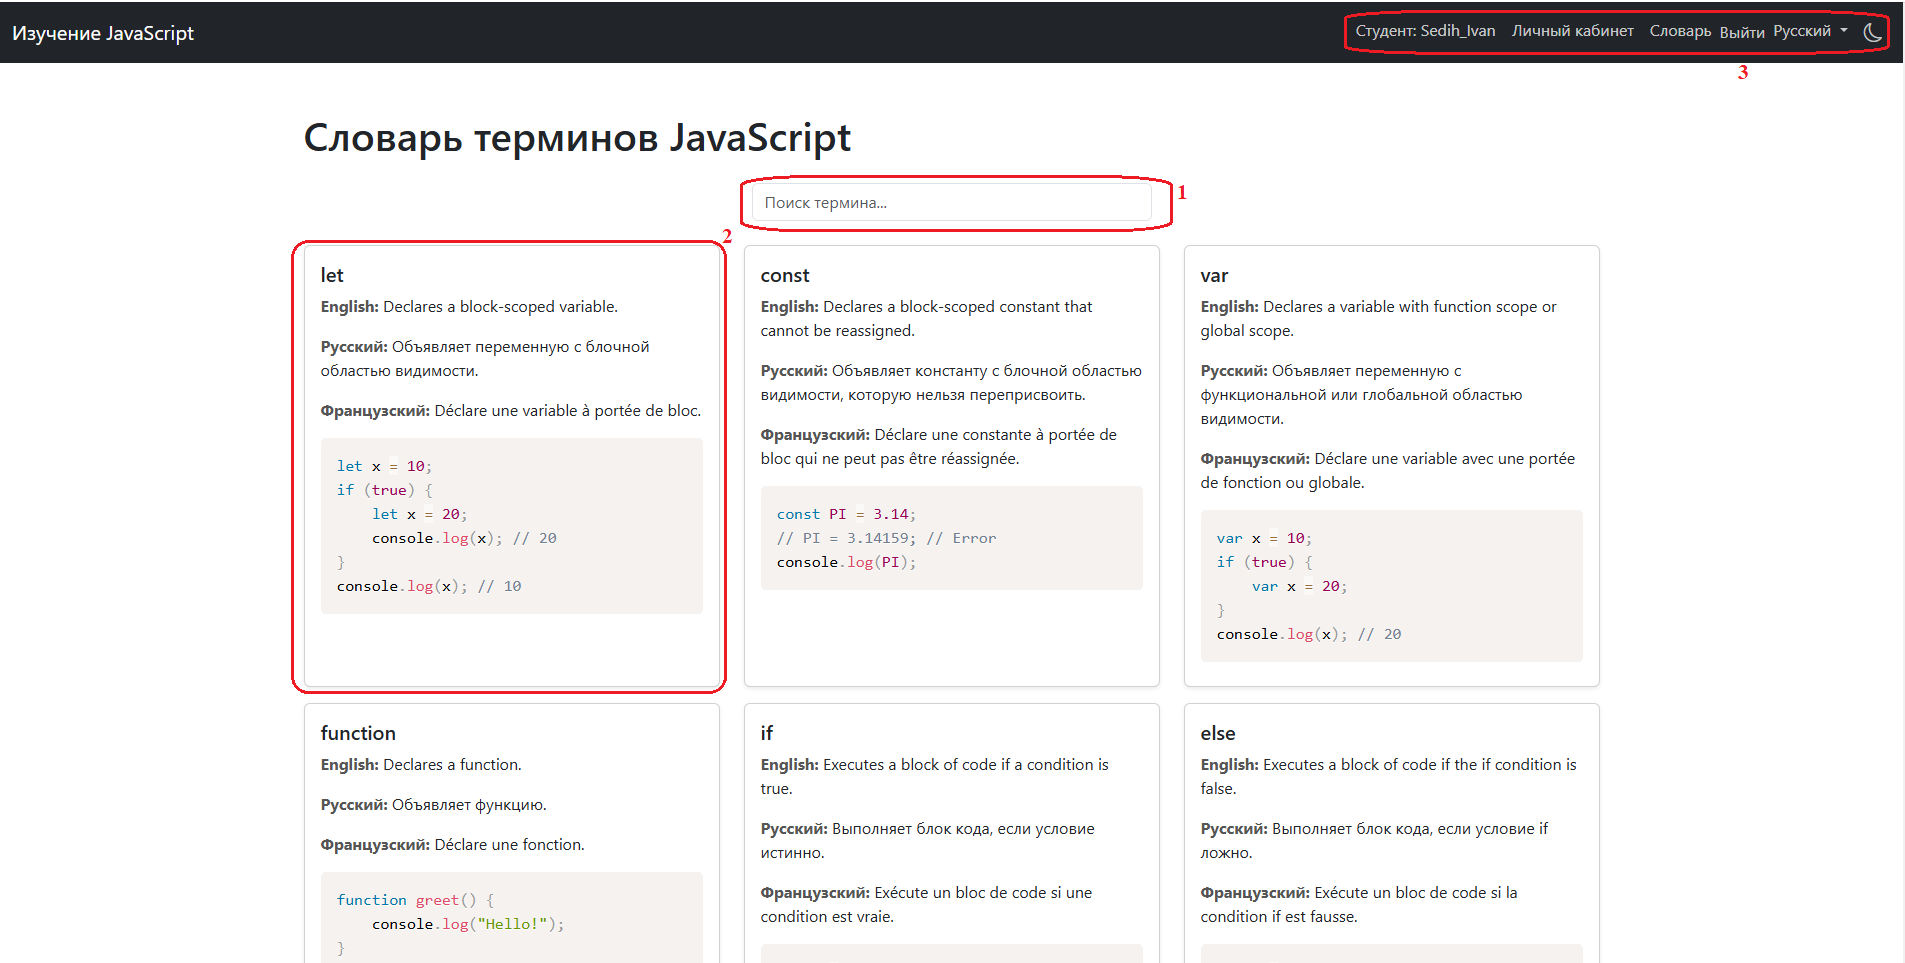
\includegraphics[width=1\linewidth]{images/словарь}
	\caption{Композиция интерфейса сервиса <<Словарь>>}
	\label{templ:image10}
\end{figure}

Композиция шаблона создание курса представлена на рисунке ~\ref{templ:image11} и состоит из:

\begin{itemize}
	\item навигационная панель (1);
	\item окно создания курса (2);
	\item поле ввода заголовка курса (3);
	\item поле ввода описания курса (4);
	\item кнопка выбора изображения (5);
	\item поле выбора статуса курса (6);
	\item кнопка сохранения курса (7);
	\item кнопка отмены (8).
\end{itemize}

\begin{figure}[h]
	\centering
	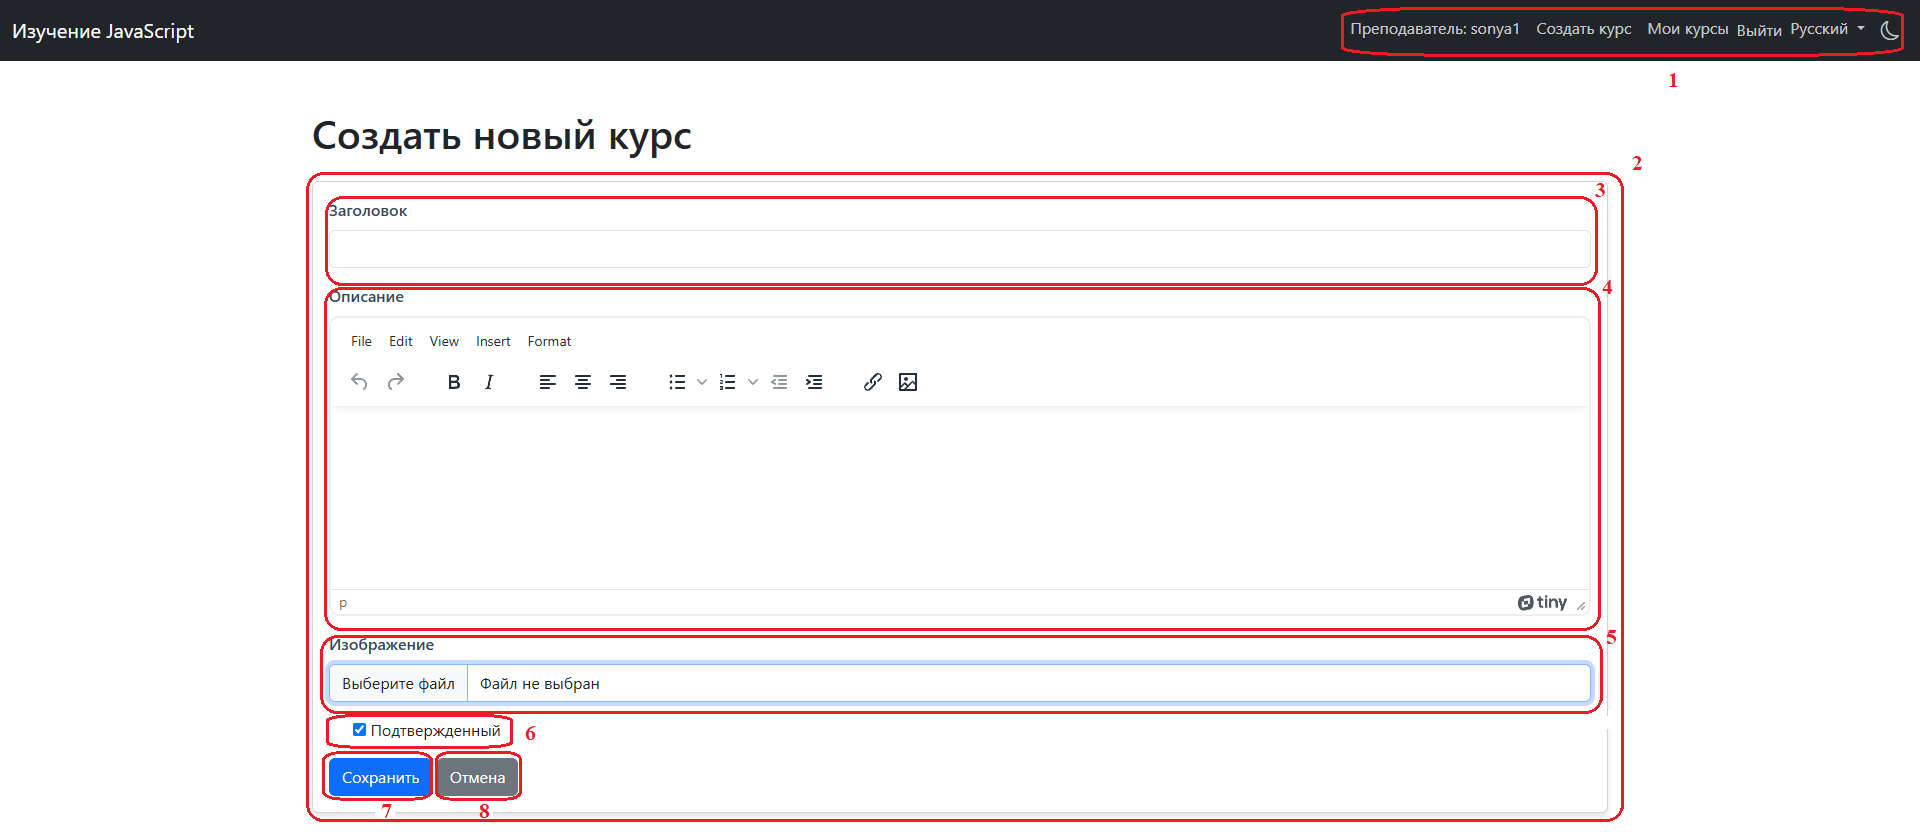
\includegraphics[width=0.9\linewidth]{images/создатькурс}
	\caption{Композиция интерфейса сервиса <<Создание курса>>}
	\label{templ:image11}
\end{figure}


Композиция шаблона создание урока представлена на рисунке ~\ref{templ:image12} и состоит из:

\begin{itemize}
	\item поле ввода заголовка урока (1);
	\item поле ввода описания урока (2);
	\item поле ввода материалов урока (3);
	\item поле ввода ссылки на видеоролик (4);
	\item поле ввода порядка урока (5);
	\item поле ввода статуса урока (6);
	\item поле ввода интерактивного задания (7);
	\item поле ввода верного ответа на задание (8);
	\item кнопка добавления урока (9);
	\item навигационная панель (10).
\end{itemize}

\begin{figure}[h]
	\centering
	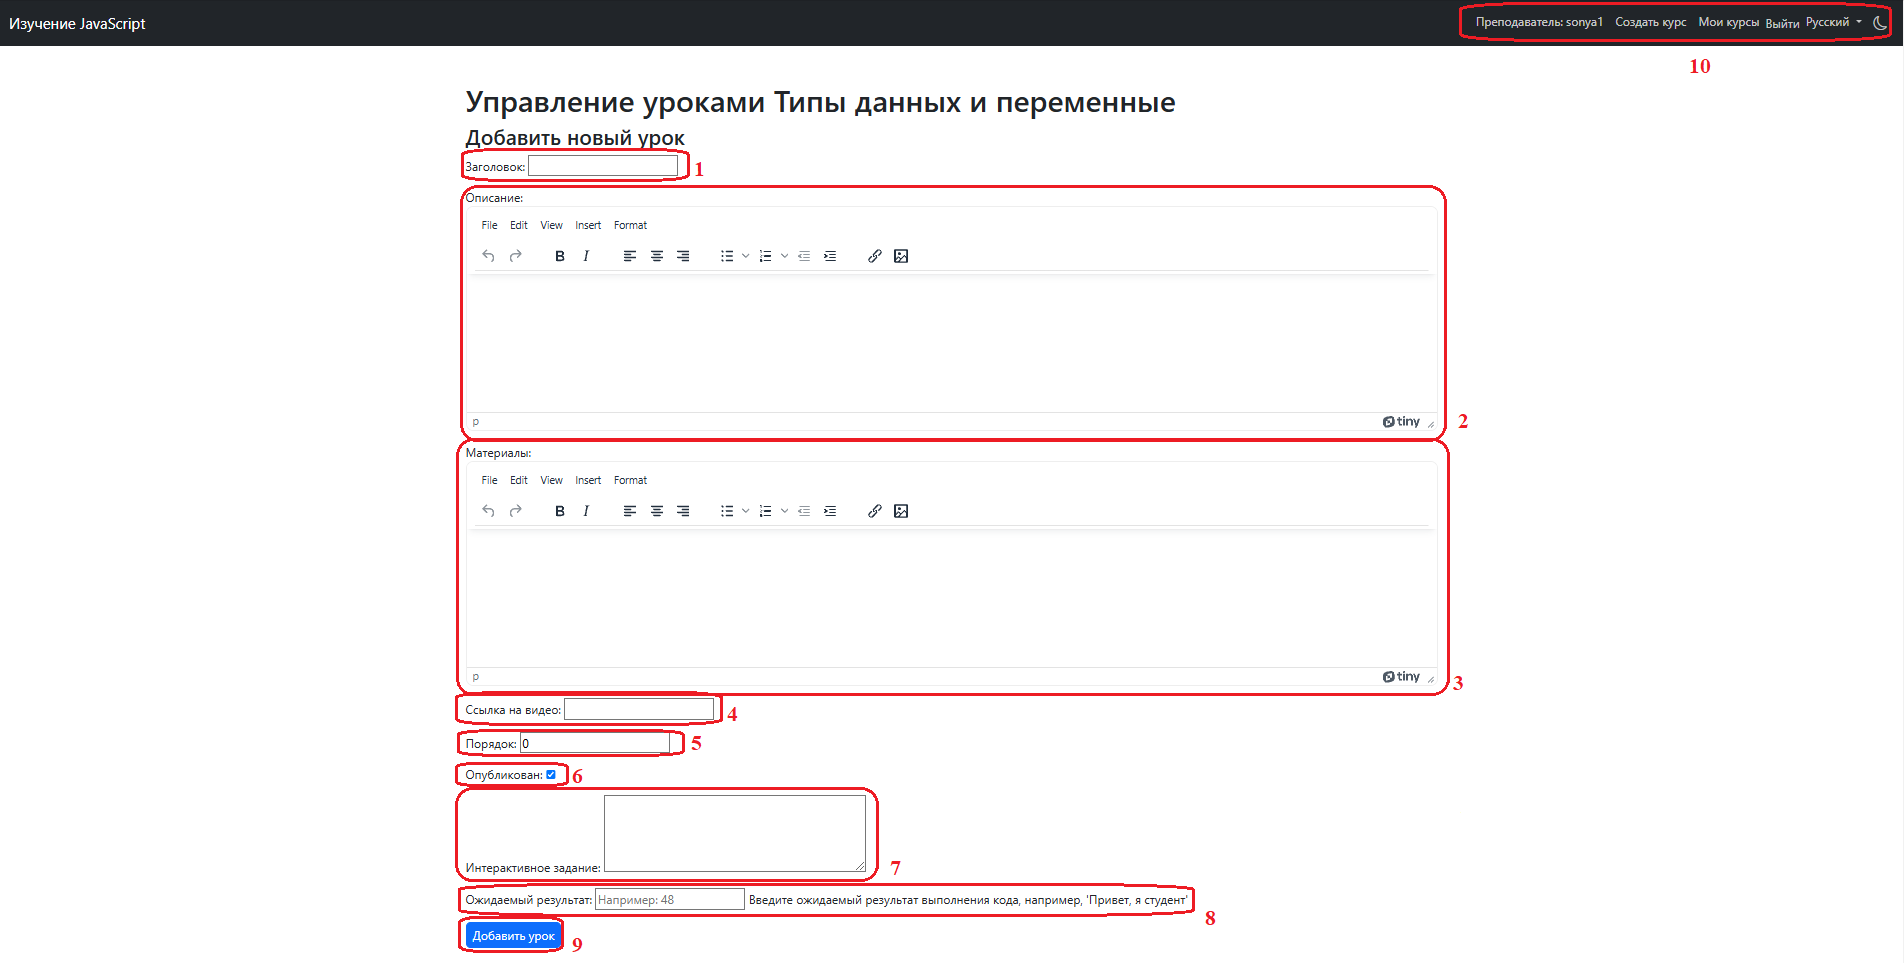
\includegraphics[width=1\linewidth]{images/создатьурок}
	\caption{Композиция интерфейса сервиса <<Создание урока>>}
	\label{templ:image12}
\end{figure}

\clearpage
\subsection{Моделирование вариантов использования}

Для разработки платформы была построена UML-диаграмма вариантов использования, отражающая взаимодействие пользователей с системой.

\begin{figure}[H]
	\centering
	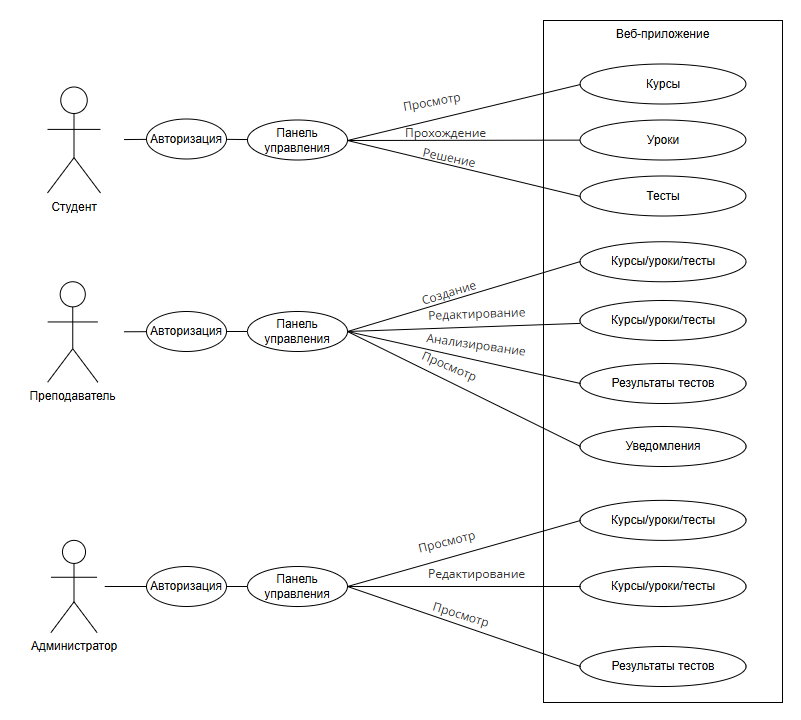
\includegraphics[width=\linewidth]{images/UML}
	\caption{Диаграмма прецедентов}
	\label{fig:usecase_diagram}
\end{figure}

Основные варианты использования системы:

\begin{enumerate}
	\item Авторизация и выход из системы: позволяет пользователям (преподавателям, студентам, администраторам) входить в систему и выходить из неё.
	\item Регистрация пользователей: обеспечивает создание учётных записей для студентов и преподавателей.
	\item Управление курсами: обеспечивает создание, редактирование и удаление курсов преподавателями, а также просмотр и запись на курсы студентами.
	\item Управление уроками: даёт возможность преподавателям управлять уроками, а студентам — изучать их материалы.
	\item Создание и управление тестами: позволяет преподавателям создавать тесты, а студентам — проходить их.
	\item Прохождение тестов: обеспечивает студентам возможность проходить тесты с автоматической оценкой.
	\item Просмотр результатов тестов: позволяет преподавателям и студентам анализировать результаты.
	\item Отслеживание прогресса: позволяет студентам видеть свой прогресс, а преподавателям — анализировать успеваемость.
	\item Управление достижениями: обеспечивает создание достижений администраторами и их получение студентами.
	\item Управление пользователями: позволяет администраторам редактировать или удалять пользователей и назначать роли.
	\item Редактирование профиля: даёт пользователям возможность обновлять свои данные.
	\item Поиск курсов: позволяет студентам находить курсы по ключевым словам или фильтрам.
	\item Локализация интерфейса: обеспечивает переключение языка интерфейса для удобства пользователей.
	\item Получение уведомлений: информирует пользователей о действиях и ошибках.
\end{enumerate}

После авторизации пользователь переходит на главную страницу: преподаватели видят панель управления, студенты — список доступных курсов, администраторы — административную панель. Ниже приведено подробное описание каждого сервиса и связанных прецедентов.

\subsubsection{Сервис <<Авторизация>>}

{Прецедент: авторизация и выход из системы}. \\
{Цель}: вход в систему и завершение сеанса. \\
{Актёр}: пользователь (преподаватель, студент, администратор). \\
{Предусловие}: пользователь зарегистрирован. \\
{Основной сценарий}:
\begin{itemize}
	\item пользователь переходит на страницу авторизации;
	\item вводит username и password;
	\item система проверяет данные в таблице coursesuser;
	\item при успешной авторизации пользователь перенаправляется на главную страницу;
	\item для выхода пользователь нажимает кнопку <<Выйти>>, система завершает сеанс.
\end{itemize}
{Постусловие}: пользователь авторизован или вышел из системы. \\
{Альтернативный сценарий}: если данные неверны, система выдаёт уведомление об ошибке.

\subsubsection{Сервис <<Регистрация>>}

{Прецедент: регистрация пользователей}. \\
{Цель}: создание учётной записи для студентов или преподавателей. \\
{Актёр}: незарегистрированный пользователь. \\
{Предусловие}: пользователь находится на странице регистрации. \\
{Основной сценарий}:
\begin{itemize}
	\item пользователь выбирает роль (студент или преподаватель);
	\item заполняет форму: username, email, password, isstudent или isteacher;
	\item система валидирует данные через StudentSignUpForm или TeacherSignUpForm;
	\item при успешной регистрации пользователь добавляется в таблицу coursesuser;
	\item пользователь перенаправляется на страницу авторизации.
\end{itemize}
{Постусловие}: учётная запись создана, данные сохранены в базе. \\
{Альтернативный сценарий}: если username или email заняты, система выдаёт уведомление об ошибке.

\subsubsection{Сервис <<Курсы>>}

{Прецедент: управление курсами (для преподавателей)}. \\
{Цель}: создание, редактирование и удаление курсов. \\
{Актёр}: преподаватель. \\
{Предусловие}: преподаватель авторизован и находится в панели управления. \\
{Основной сценарий}:
\begin{itemize}
	\item преподаватель переходит в раздел <<Курсы>>;
	\item нажимает кнопку <<Создать курс>>;
	\item заполняет форму: название (title), описание (description), изображение (image), статус активности (isactive);
	\item сохраняет курс, система добавляет его в таблицу coursescourse и связывает с преподавателем (creator);
	\item для редактирования или удаления преподаватель выбирает курс из списка и выполняет действие.
\end{itemize}
{Постусловие}: курс создан, отредактирован или удалён, изменения отражены в базе данных. \\
{Альтернативный сценарий}: если форма заполнена некорректно (например, пустое название), система выдаёт уведомление об ошибке.

{Прецедент: просмотр и запись на курсы (для студентов)}. \\
{Цель}: просмотр доступных курсов и запись на них. \\
{Актёр}: студент. \\
{Предусловие}: студент авторизован. \\
{Основной сценарий}:
\begin{itemize}
	\item студент переходит на главную страницу, где отображается список курсов;
	\item список включает название, описание и статус курса (например, <<Доступен>>, <<Завершён>>);
	\item студент выбирает курс и нажимает кнопку <<Записаться>>;
	\item система добавляет запись в таблицу coursesenrollment с полями course, student, enrolledat.
\end{itemize}
{Постусловие}: студент записан на курс, запись отражена в базе данных. \\
{Альтернативный сценарий}: если студент уже записан, система уведомляет об этом.

{Прецедент: поиск курсов (для студентов)}. \\
{Цель}: поиск курсов по ключевым словам или фильтрам. \\
{Актёр}: студент. \\
{Предусловие}: студент авторизован. \\
{Основной сценарий}:
\begin{itemize}
	\item студент переходит на страницу курсов;
	\item вводит запрос в поле поиска (например, <<JavaScript>>) или выбирает фильтры (например, <<Активные курсы>>);
	\item система выполняет поиск по полю title в таблице coursescourse;
	\item отображается список подходящих курсов.
\end{itemize}
{Постусловие}: студент получил список курсов, соответствующих запросу. \\
{Альтернативный сценарий}: если курсы не найдены, отображается сообщение <<Курсы не найдены>>.

\subsubsection{Сервис <<Уроки>>}

{Прецедент: управление уроками (для преподавателей)}. \\
{Цель}: добавление, редактирование, сортировка и удаление уроков в рамках курса. \\
{Актёр}: преподаватель. \\
{Предусловие}: преподаватель авторизован, выбран курс. \\
{Основной сценарий}:
\begin{itemize}
	\item преподаватель переходит в раздел <<Уроки>> выбранного курса;
	\item нажимает кнопку <<Добавить урок>>;
	\item заполняет форму: название (title), описание (description), содержимое (content), ссылка на видео (videourl), порядок (order), статус публикации (ispublished);
	\item сохраняет урок, система добавляет его в таблицу courseslesson;
	\item для сортировки использует интерфейс с Sortable.js, изменяя поле order;
	\item для редактирования или удаления выбирает урок из списка;
	\item может включить предпросмотр урока перед публикацией.
\end{itemize}
{Постусловие}: урок добавлен, отредактирован, отсортирован или удалён. \\
{Альтернативный сценарий}: если videourl недействителен, система уведомляет об ошибке.

{Прецедент: изучение уроков (для студентов)}. \\
{Цель}: просмотр материалов урока. \\
{Актёр}: студент. \\
{Предусловие}: студент записан на курс, урок опубликован. \\
{Основной сценарий}:
\begin{itemize}
	\item студент выбирает курс и переходит в раздел <<Уроки>>;
	\item видит список уроков, отсортированных по полю order;
	\item выбирает урок и просматривает материалы: текст (content), видео (videourl);
	\item после завершения урока система обновляет прогресс в таблице coursesstudentprogress: completed.
\end{itemize}
{Постусловие}: урок изучен, прогресс обновлён. \\
{Альтернативный сценарий}: если урок не опубликован, он недоступен для просмотра.

\subsubsection{Сервис <<Тесты>>}

{Прецедент: создание и управление тестами (для преподавателей)}. \\
{Цель}: создание тестов с вопросами и ответами. \\
{Актёр}: преподаватель. \\
{Предусловие}: преподаватель авторизован, выбран урок. \\
{Основной сценарий}:
\begin{itemize}
	\item преподаватель переходит в раздел <<Тесты>> урока;
	\item нажимает кнопку <<Создать тест>>;
	\item заполняет форму: название (title), описание (description), проходной балл (passingscore), статус (isactive);
	\item добавляет вопросы в таблицу coursesquestion: текст (text), тип (questiontype), баллы (points);
	\item для каждого вопроса добавляет варианты ответа в таблицу coursesanswer: текст (text), правильность (iscorrect), порядок (order);
	\item сохраняет тест, система добавляет его в таблицу coursestest.
\end{itemize}
{Постусловие}: тест создан и связан с уроком (lesson). \\
{Альтернативный сценарий}: если passingscore некорректен, система выдаёт ошибку.

{Прецедент: прохождение тестов (для студентов)}. \\
{Цель}: прохождение теста и получение оценки. \\
{Актёр}: студент. \\
{Предусловие}: студент записан на курс, тест активен. \\
{Основной сценарий}:
\begin{itemize}
	\item студент переходит к уроку и выбирает тест;
	\item система отображает вопросы с вариантами ответов;
	\item студент выбирает ответы и отправляет тест;
	\item система оценивает ответы, сравнивая с iscorrect, и сохраняет результат в таблице coursestestresult: score, answers, attempts.
\end{itemize}
{Постусловие}: тест пройден, результат сохранён. \\
{Альтернативный сценарий}: если тест неактивен, он недоступен.

\subsubsection{Сервис <<Результаты тестов>>}

{Прецедент: просмотр и анализ результатов (для преподавателей)}. \\
{Цель}: анализ успеваемости студентов. \\
{Актёр}: преподаватель. \\
{Предусловие}: преподаватель авторизован, тест пройден хотя бы одним студентом. \\
{Основной сценарий}:
\begin{itemize}
	\item преподаватель переходит в раздел <<Результаты тестов>>;
	\item система отображает список студентов, их баллы (score), количество попыток (attempts) и ответы (answers);
	\item преподаватель может удалить результат, если он некорректен.
\end{itemize}
{Постусловие}: преподаватель получил статистику по тесту. \\
{Альтернативный сценарий}: если результатов нет, отображается сообщение <<Нет данных>>.

{Прецедент: просмотр результатов (для студентов)}. \\
{Цель}: просмотр своих баллов и статистики. \\
{Актёр}: студент. \\
{Предусловие}: студент прошёл тест. \\
{Основной сценарий}:
\begin{itemize}
	\item студент переходит в раздел <<Результаты>>;
	\item система отображает баллы (score), количество попыток (attempts) и правильные/неправильные ответы.
\end{itemize}
{Постусловие}: студент увидел свои результаты. \\
{Альтернативный сценарий}: если тест не пройден, результаты недоступны.

\subsubsection{Сервис <<Прогресс>>}

{Прецедент: отслеживание прогресса (для студентов)}. \\
{Цель}: просмотр прогресса по курсу и урокам. \\
{Актёр}: студент. \\
{Предусловие}: студент записан на курс. \\
{Основной сценарий}:
\begin{itemize}
	\item студент переходит в раздел <<Мой прогресс>>;
	\item система отображает список курсов и уроков с состоянием completed из таблицы coursesstudentprogress;
	\item отображается процент завершения курса на основе завершённых уроков.
\end{itemize}
{Постусловие}: студент увидел свой прогресс. \\
{Альтернативный сценарий}: если прогресс отсутствует, отображается сообщение <<Прогресс не начат>>.

{Прецедент: анализ прогресса (для преподавателей)}. \\
{Цель}: анализ прогресса студентов по курсу. \\
{Актёр}: преподаватель. \\
{Предусловие}: преподаватель авторизован, курс имеет записанных студентов. \\
{Основной сценарий}:
\begin{itemize}
	\item преподаватель переходит в раздел <<Прогресс студентов>>;
	\item система отображает список студентов и их прогресс (completed, completedat) из таблицы coursesstudentprogress;
	\item преподаватель может фильтровать данные по курсу или студенту.
\end{itemize}
{Постусловие}: преподаватель получил статистику прогресса. \\
{Альтернативный сценарий}: если данных нет, отображается сообщение <<Нет данных>>.

\subsubsection{Сервис <<Достижения>>}

{Прецедент: управление достижениями (для администраторов)}. \\
{Цель}: создание и редактирование достижений. \\
{Актёр}: администратор. \\
{Предусловие}: администратор авторизован. \\
{Основной сценарий}:
\begin{itemize}
	\item администратор переходит в раздел <<Достижения>>;
	\item нажимает кнопку <<Создать достижение>>;
	\item заполняет форму: название (title), описание (description);
	\item сохраняет достижение, система добавляет его в таблицу coursesachievement;
	\item для редактирования или удаления выбирает достижение из списка.
\end{itemize}
{Постусловие}: достижение создано или отредактировано. \\
{Альтернативный сценарий}: если title не уникален, система выдаёт ошибку.

{Прецедент: получение достижений (для студентов)}. \\
{Цель}: просмотр и получение достижений. \\
{Актёр}: студент. \\
{Предусловие}: студент выполнил условие для достижения (например, завершил урок). \\
{Основной сценарий}:
\begin{itemize}
	\item система автоматически проверяет условия достижения (например, completed в coursesstudentprogress);
	\item при выполнении условия добавляет запись в таблицу coursesuserachievement: user, achievement, awardedat;
	\item студент видит достижение в разделе <<Мои достижения>>.
\end{itemize}
{Постусловие}: студент получил достижение. \\
{Альтернативный сценарий}: если условия не выполнены, достижение не присваивается.

\subsubsection{Сервис <<Пользователи>>}

{Прецедент: управление пользователями (для администраторов)}. \\
{Цель}: редактирование, удаление пользователей и назначение ролей. \\
{Актёр}: администратор. \\
{Предусловие}: администратор авторизован. \\
{Основной сценарий}:
\begin{itemize}
	\item администратор переходит в раздел <<Пользователи>>;
	\item система отображает список пользователей из таблицы coursesuser;
	\item администратор выбирает пользователя и редактирует поля (username, email, isstudent, isteacher) или удаляет его;
	\item изменения сохраняются в базе данных.
\end{itemize}
{Постусловие}: данные пользователя обновлены или удалены. \\
{Альтернативный сценарий}: если пользователь связан с курсами, удаление блокируется.

\subsubsection{Сервис <<Профиль>>}

{Прецедент: редактирование профиля}. \\
{Цель}: обновление данных пользователя. \\
{Актёр}: пользователь (преподаватель, студент). \\
{Предусловие}: пользователь авторизован. \\
{Основной сценарий}:
\begin{itemize}
	\item пользователь переходит в раздел <<Профиль>>;
	\item заполняет форму: email, password, firstname, lastname;
	\item система валидирует данные через формы Django;
	\item изменения сохраняются в таблице coursesuser.
\end{itemize}
{Постусловие}: профиль обновлён. \\
{Альтернативный сценарий}: если данные некорректны (например, неверный формат email), система выдаёт ошибку.

\subsubsection{Сервис <<Локализация>>}

{Прецедент: локализация интерфейса}. \\
{Цель}: переключение языка интерфейса. \\
{Актёр}: любой пользователь (преподаватель, студент). \\
{Предусловие}: пользователь авторизован. \\
{Основной сценарий}:
\begin{itemize}
	\item пользователь выбирает язык (например, русский или английский) в меню настроек;
	\item система использует Django i18n для переключения языка интерфейса;
	\item страница обновляется с новым языком, включая текст интерфейса и вопросы тестов.
\end{itemize}
{Постусловие}: язык интерфейса изменён. \\
{Альтернативный сценарий}: если выбранный язык недоступен, система уведомляет об ошибке.

\subsubsection{Сервис <<Уведомления>>}

{Прецедент: получение уведомлений}. \\
{Цель}: информирование о действиях и ошибках. \\
{Актёр}: любой пользователь. \\
{Предусловие}: пользователь выполнил действие (например, добавил урок). \\
{Основной сценарий}:
\begin{itemize}
	\item после действия (например, добавления урока) система генерирует уведомление (<<Урок успешно добавлен>>);
	\item уведомление отображается в интерфейсе (например, в верхней части страницы);
	\item при ошибке (например, некорректный формат данных) отображается сообщение об ошибке.
\end{itemize}
{Постусловие}: пользователь получил уведомление. \\
{Альтернативный сценарий}: если уведомления отключены, сообщение не отображается.

\subsubsection{Сервис <<Панель управления>>}

{Прецедент: доступ к панели управления (для преподавателей)}. \\
{Цель}: быстрый доступ к функциям управления. \\
{Актёр}: преподаватель. \\
{Предусловие}: преподаватель авторизован. \\
{Основной сценарий}:
\begin{itemize}
	\item после авторизации преподаватель переходит на главную страницу;
	\item панель управления отображает виджеты: список курсов, уроки, тесты, результаты;
	\item преподаватель переходит к нужному разделу (например, <<Курсы>>).
\end{itemize}
{Постусловие}: преподаватель получил доступ к функциям управления. \\
{Альтернативный сценарий}: если доступ ограничен, отображается ошибка.

{Прецедент: доступ к списку курсов (для студентов)}. \\
{Цель}: просмотр доступных курсов. \\
{Актёр}: студент. \\
{Предусловие}: студент авторизован. \\
{Основной сценарий}:
\begin{itemize}
	\item после авторизации студент переходит на главную страницу;
	\item система отображает список доступных курсов;
	\item студент выбирает курс для изучения.
\end{itemize}
{Постусловие}: студент получил доступ к курсам. \\
{Альтернативный сценарий}: если курсы отсутствуют, отображается сообщение <<Нет доступных курсов>>.


\subsection{Требования к оформлению документации}

Разработка программной документации и программного изделия должна производиться согласно ГОСТ 19.102–77 и ГОСТ 34.601–90. Единая система программной документации.
